\documentclass[a4paper,twoside]{article}
\usepackage{array}
\newcolumntype{C}[1]{>{\centering\let\newline\\\arraybackslash\hspace{0pt}}m{#1}}
\usepackage{amsfonts}
\usepackage{amsmath}
\usepackage{graphicx}
\usepackage{caption}
\usepackage{subcaption}
\hyphenation{op-tical net-works semi-conduc-tor}
\usepackage{color}
\usepackage{epsfig}
\usepackage{subcaption}
\usepackage{calc}
\usepackage{amssymb}
\usepackage{amstext}
\usepackage{amsmath}
\usepackage{amsthm}
\usepackage{multicol}
\usepackage{pslatex}
\usepackage{apalike}
\usepackage{SCITEPRESS}     % Please add other packages that you may need BEFORE the SCITEPRESS.sty package.


\begin{document}
	
	\title{Road Tracking Using Deep Reinforcement Learning for Driving Cars Applications}
	
	\author{\authorname{Raid R. O. Al-Nima\sup{1}\orcidAuthor{0000-1111-2222-3333}, Tingting Han\sup{2}\orcidAuthor{1111-2222-3333-4444} and Taolue Chen\sup{2}\orcidAuthor{2222-3333-4444-5555}}
		\affiliation{\sup{1}Technical Engineering College of Mosul, Northern Technical University, Iraq}
		\affiliation{\sup{2}Department of Computer Science and Information Systems, Birkbeck, University of London}
		\email{\{tingting,t.chen\}@dcs.bbk.ac.uk}}
	
	\keywords{Deep Reinforcement Learning}
	
	\abstract{Deep reinforcement learning has recently aroused wide attentions. It combines deep learning with reinforcement learning to solve difficult tasks. This paper proposes an efficient deep reinforcement learning network to solve road tracking problems. The network collects input states from forward car facing views and produces suitable road tracking actions. The actions are derived from encoding the tracking directions and movements. We explored both value iteration and policy iteration based deep reinforcement learning algorithms. A comparison between the two and a comparison with existing networks are provided. Our results are very promising - the best driving accuracy achieved 93.94\%, the highest in the comparison.}
	
	\onecolumn \maketitle \normalsize \setcounter{footnote}{0} \vfill
	
\section{\uppercase{Introduction}}
% no \IEEEPARstart
Road tracking is one of the most challenging topics recently. It aims to automatically guide a car through the correct track without crashing other cars or objects. Deep reinforcement learning is considered as one of the most proficient methods that can be applied to address the road tracking issue. It combines reinforcement learning and deep learning. We model the process as a Markov Decision Process (MDP), where the deep reinforcement learning starts from a state, pick the best action by optimising considered rewards and produces a new state. The new state is then utilized as a current state, and the process continues.  

Different tracking tasks were considered in the literature as:
\begin{itemize}
	\item \underline{Tracking Object:} In 2000, Grigore and Grigore proposed a tracking system controller by using a recurrent neural network with the reinforcement learning \cite{Grigore2000Reinforcement}. In 2010, Cohen and Pavlovic suggested an effective and vigorous real-time tracker. The tracker utilized the reinforcement learning and it was applied to tracking personal faces \cite{Cohen2010Reinforcement}. In 2004, Liu and Su proposed an object tracking method by exploiting the reinforcement learning. The reinforcement learning was employed here to determine the features of the tracking object \cite{Liu2004Reinforcement}. In 2017, Supan\v{c}i\v{c} and Ramanan constructed a learning policy for tracking objects. The reinforcement learning was applied to video streams to provide on-line decision \cite{Supancic2017Tracking}. 
	\item \underline{Different Tracking Issues:} In 2009, Jinlin \textit{et al.} presented a velocity tracking control approach. The authors utilized the neuro-fuzzy technique with the Q-learning in their work \cite{Jinlin2009Neurofuzzy}. In 2011, Hall \textit{et al.} illustrated a single and double pendulum tracking model. A traditional control, Bayesian computations and reinforcement learning were employed in this publication \cite{Hall2011Reinforcement}. In 2013, Sootla \textit{et al.} described a tracking periodic gene repressilator. The fitted Q iteration algorithm was applied to one dimensional signals in this study \cite{Sootla2013On}. In 2015, Wei \textit{et al.} explained tracking a maximum power for wind speed conversion systems. In this paper, a model-free Q-learning method was exploited \cite{Wei2015Reinforcement}. 
	\item \underline{Deep Leaning Tracking:} In 2017, Perot \textit{et al.} investigated tracking roads of a driving car. A deep reinforcement learning was used \cite{Perot2017End}. The main problem in this work is that the driving car oscillates around the main road track. This is due to the selected reward in this study, where it utilized the oriented angle of the road with the car speed. In 2017 and 2018, Yun \textit{et al.} approached an action-decision network (ADNet) to track objects. The ADNet is a deep reinforcement learning network and it was applied in a quite complicated way, where a pre-trained Convolutional Neural Network (CNN) was firstly employed then the reinforcement learning was utilized \cite{Yun2017Action}\cite{Yun2018Action}. 
\end{itemize}

It can be seen from the literature that the majority of tracking studies were focused on tracking object problems as in \cite{Grigore2000Reinforcement}\cite{Cohen2010Reinforcement}\cite{Liu2004Reinforcement}\cite{Supancic2017Tracking}. Other work considered different tracking tasks such as: tracking and controlling velocity \cite{Jinlin2009Neurofuzzy}, tracking periodic gene repressilator \cite{Sootla2013On}, tracking single and double pendulum \cite{Hall2011Reinforcement}, tracking maximum powers for wind speed conversion systems \cite{Wei2015Reinforcement}. Only several studies were concentrated on utilizing the deep learning in order to address tracking issues such as \cite{Yun2017Action,Yun2018Action}. 

Our work contributes to this area by suggesting an effective road tracking procedure and employing the MDP based on the deep reinforcement learning, where states are used as inputs; rewards are utilized to evaluate the tracking policy and actions are predicted to provide new states. Efficient coding for various road tracking possibilities has been considered such as turning to the left or right and recognizing crossing object(s). This study can be exploited for driving car applications such as driverless (or automatic driving). 

After the introduction, this paper is organized as follows: Section 2 states the methodology with the theoretical concepts, Section 3 discusses the results and Section 4 concludes the paper.
\begin{figure*}[!t]
	\centering
	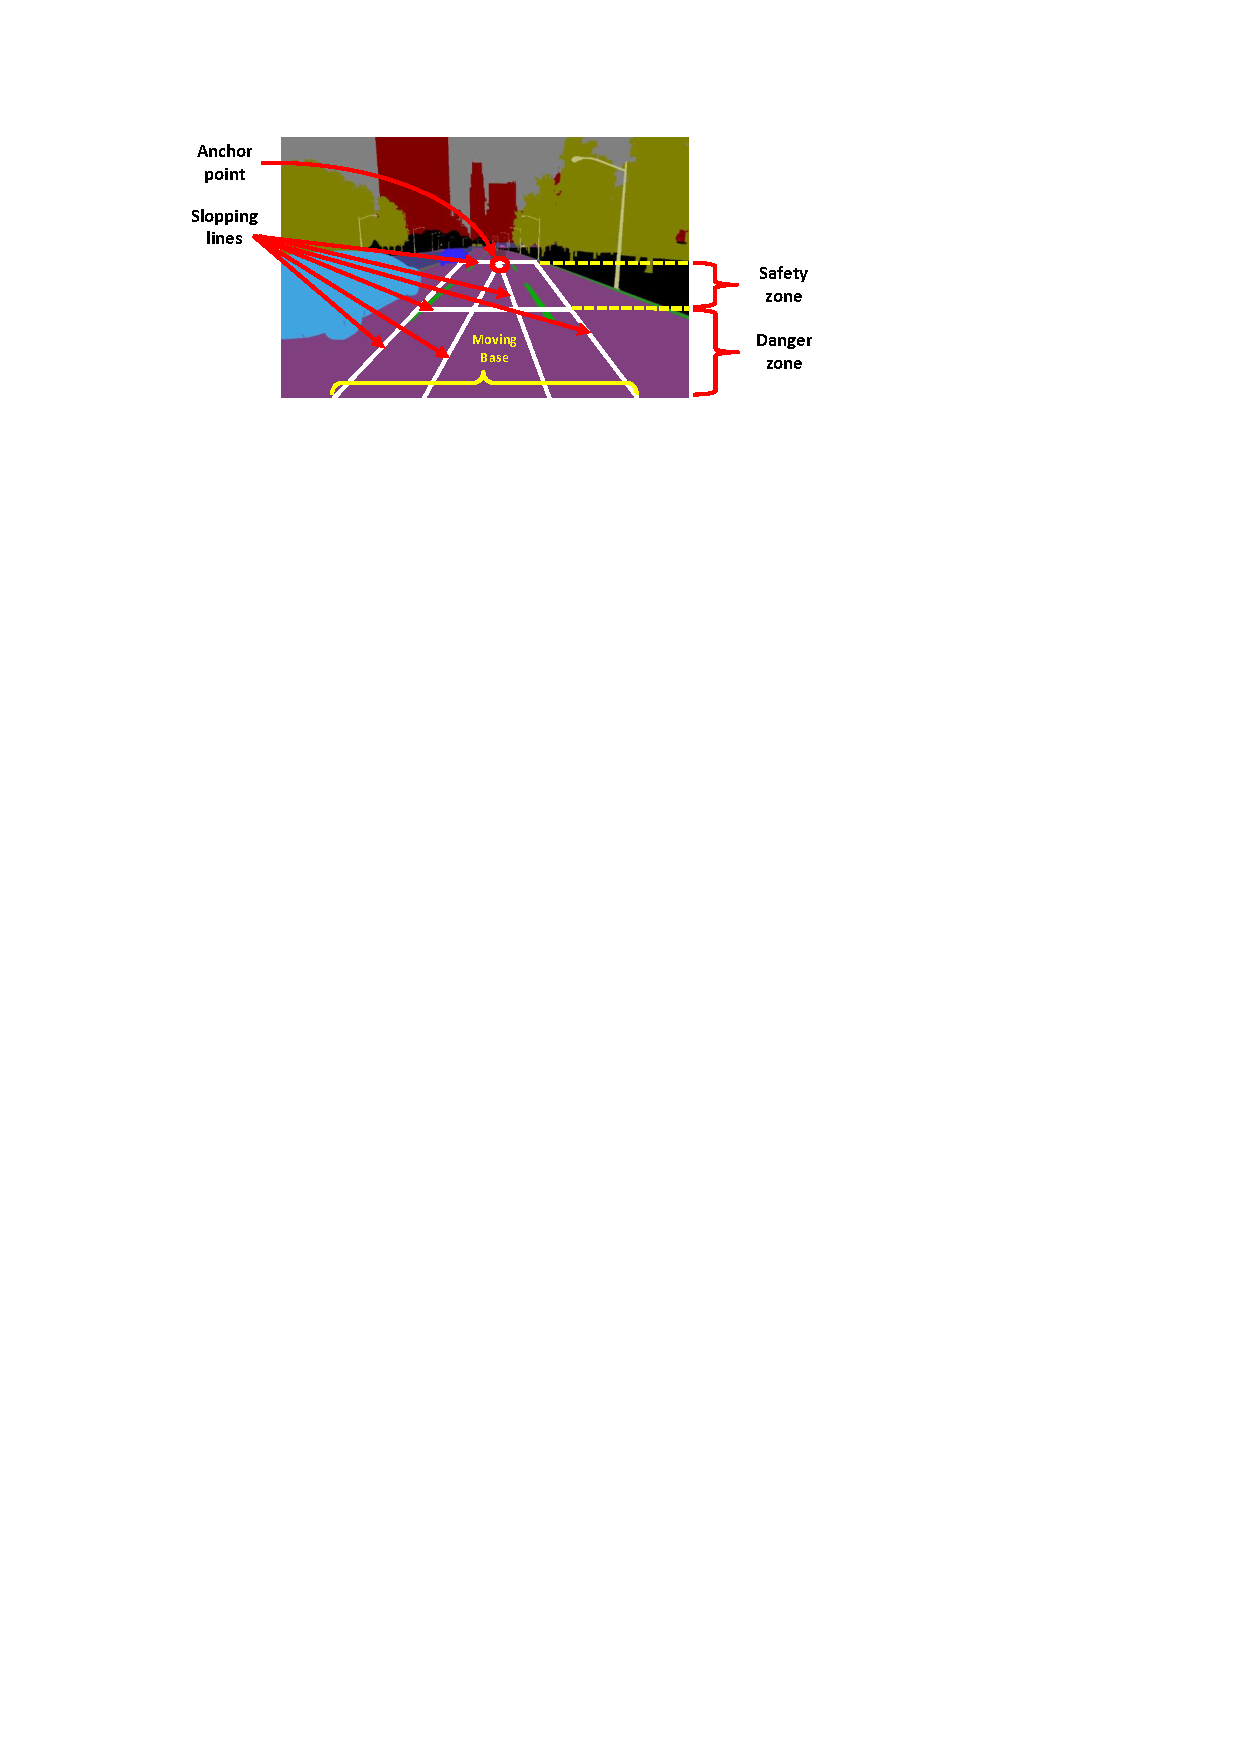
\includegraphics[scale=.9,trim=3cm 22.5cm 7.1cm 2cm,clip]{segmentation_regions2.pdf}
	\caption{The suggested front view road tracking zones, lines and anchor point}
	\label{Fig:segmentation_regions1}
\end{figure*}
\begin{figure*}[!t]
	\centering
	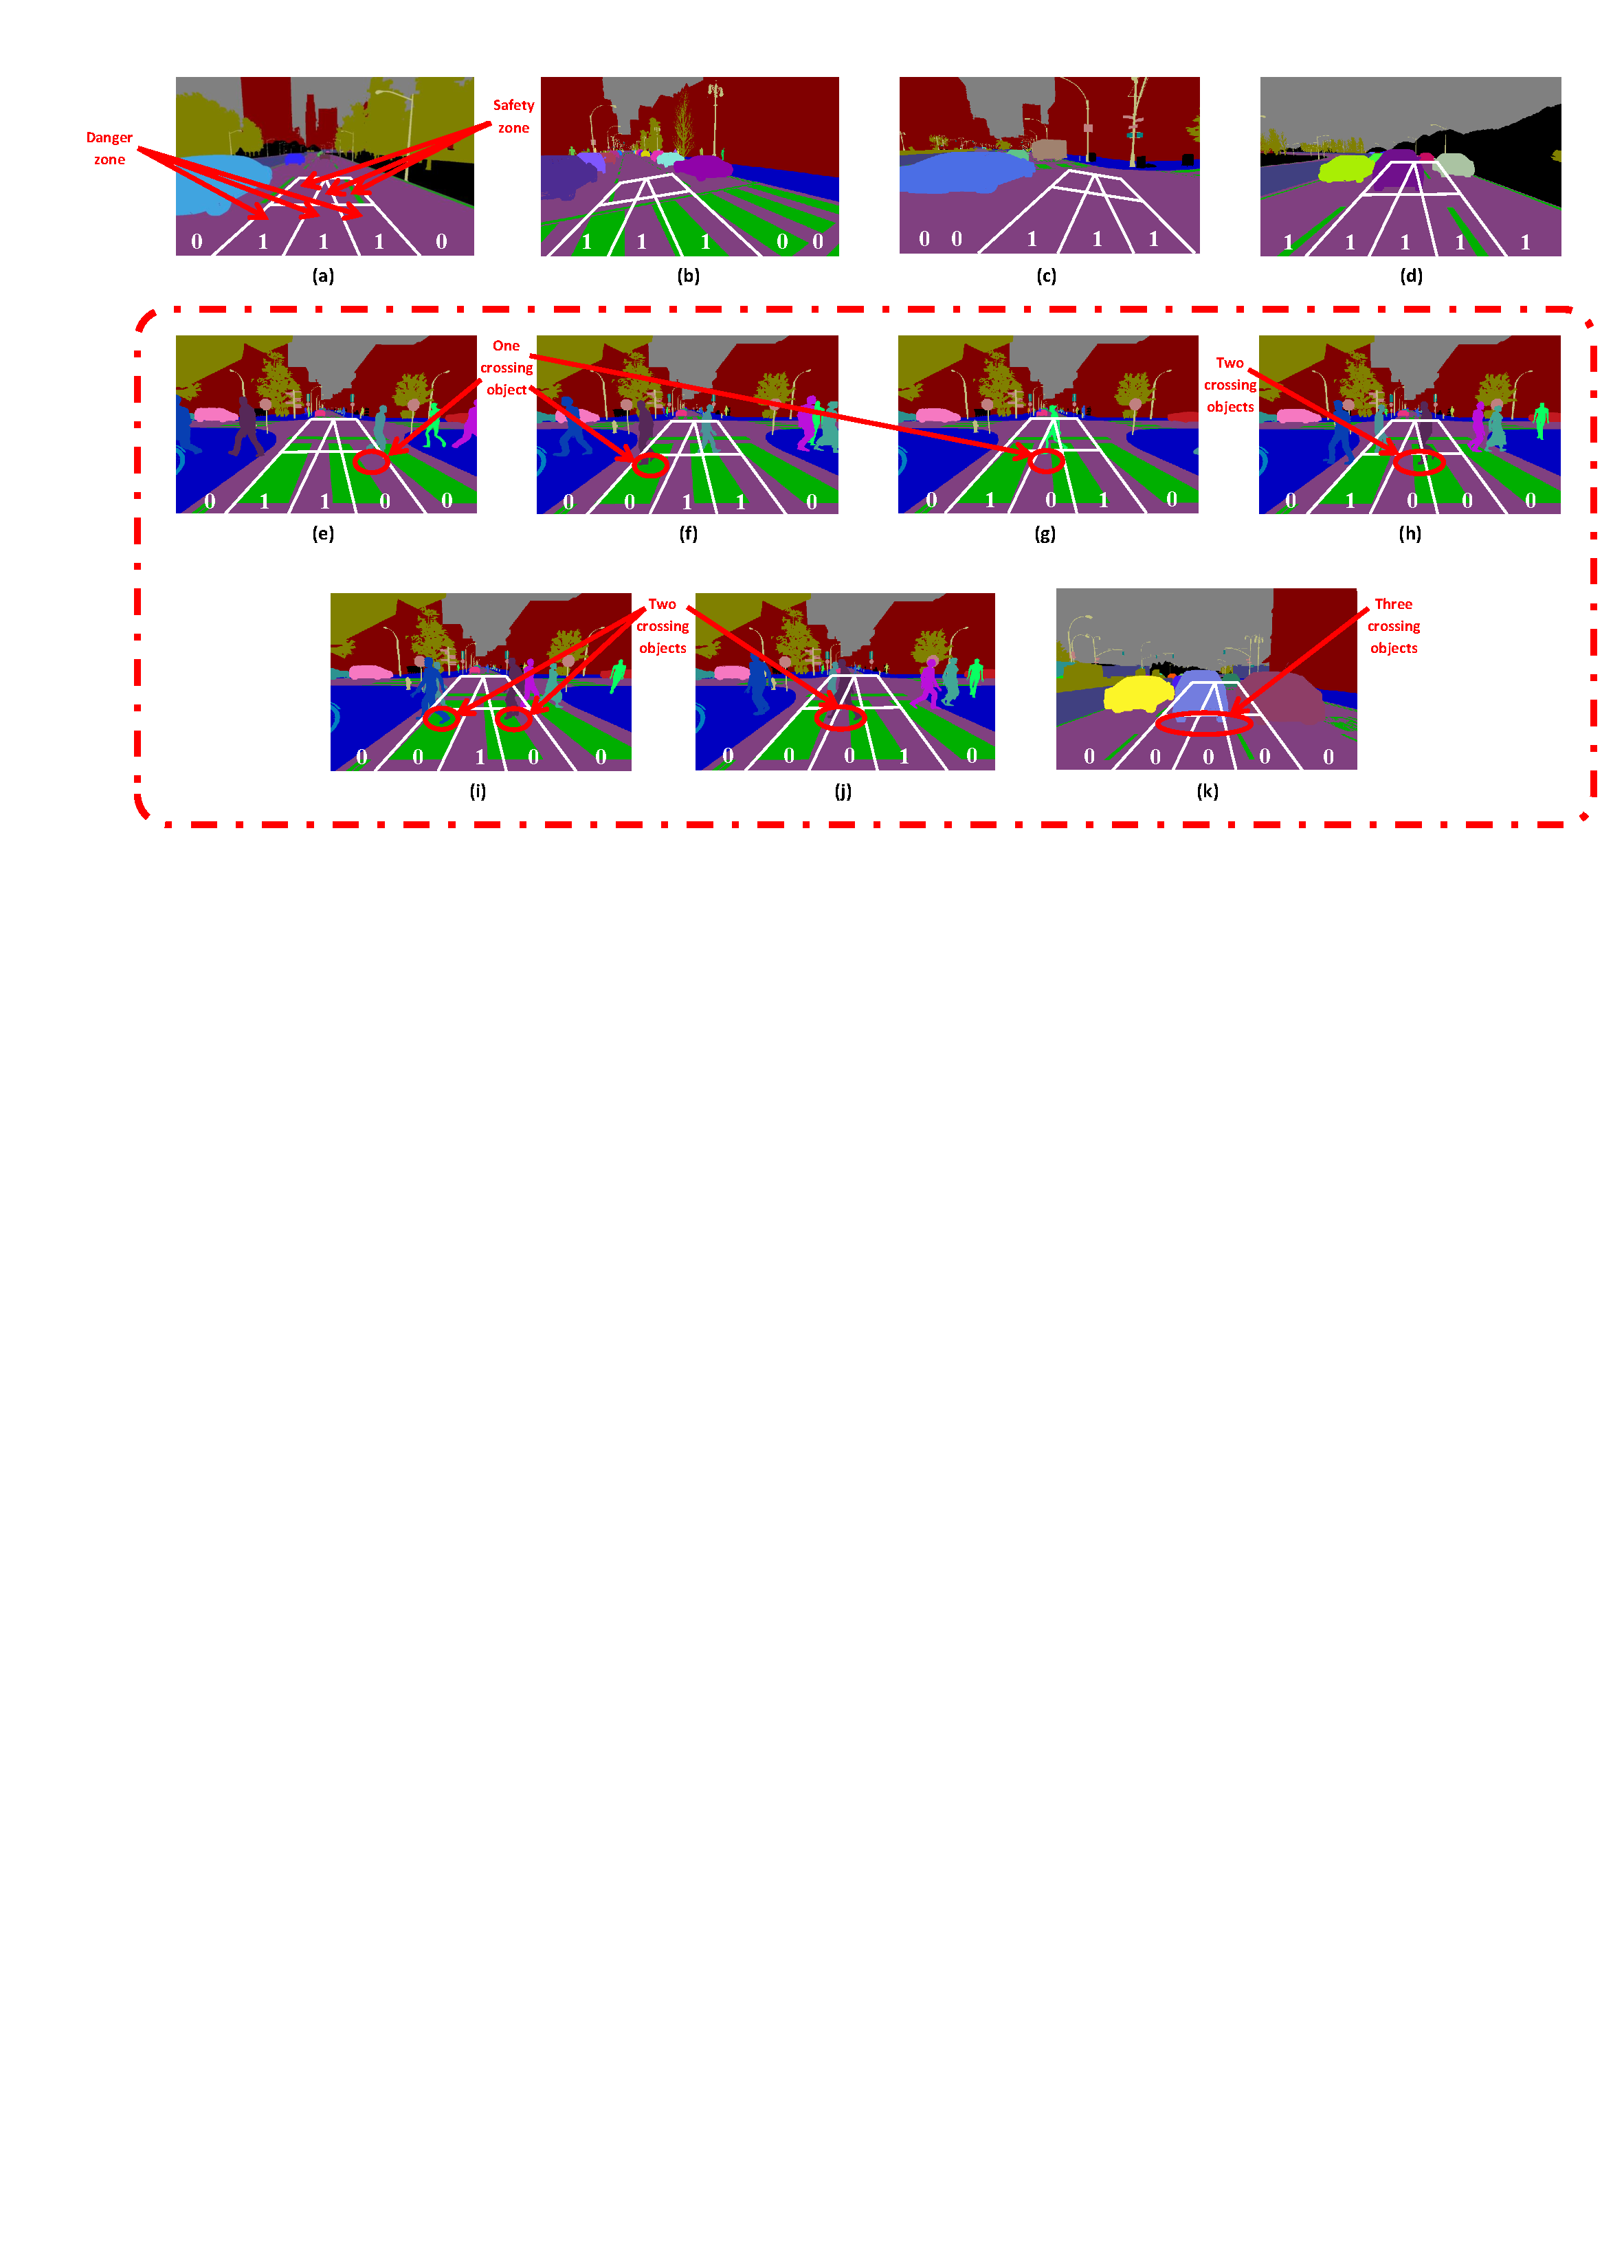
\includegraphics[scale=.4,trim=2cm 35cm 0cm 2cm,clip]{segmentation3.pdf}
	\caption{The road tracking motivations of segmented images: (a) the straight forward direction, (b) turning left direction, (c) turning right direction, (d) reverse or backward direction, (e-g) stopping action because of a single crossing object, (h-j) stopping action because of two crossing objects and (k) stopping action because of three crossing objects}
	\label{Fig:segmentation}
\end{figure*}
\begin{figure*}[!h]
	\centering
	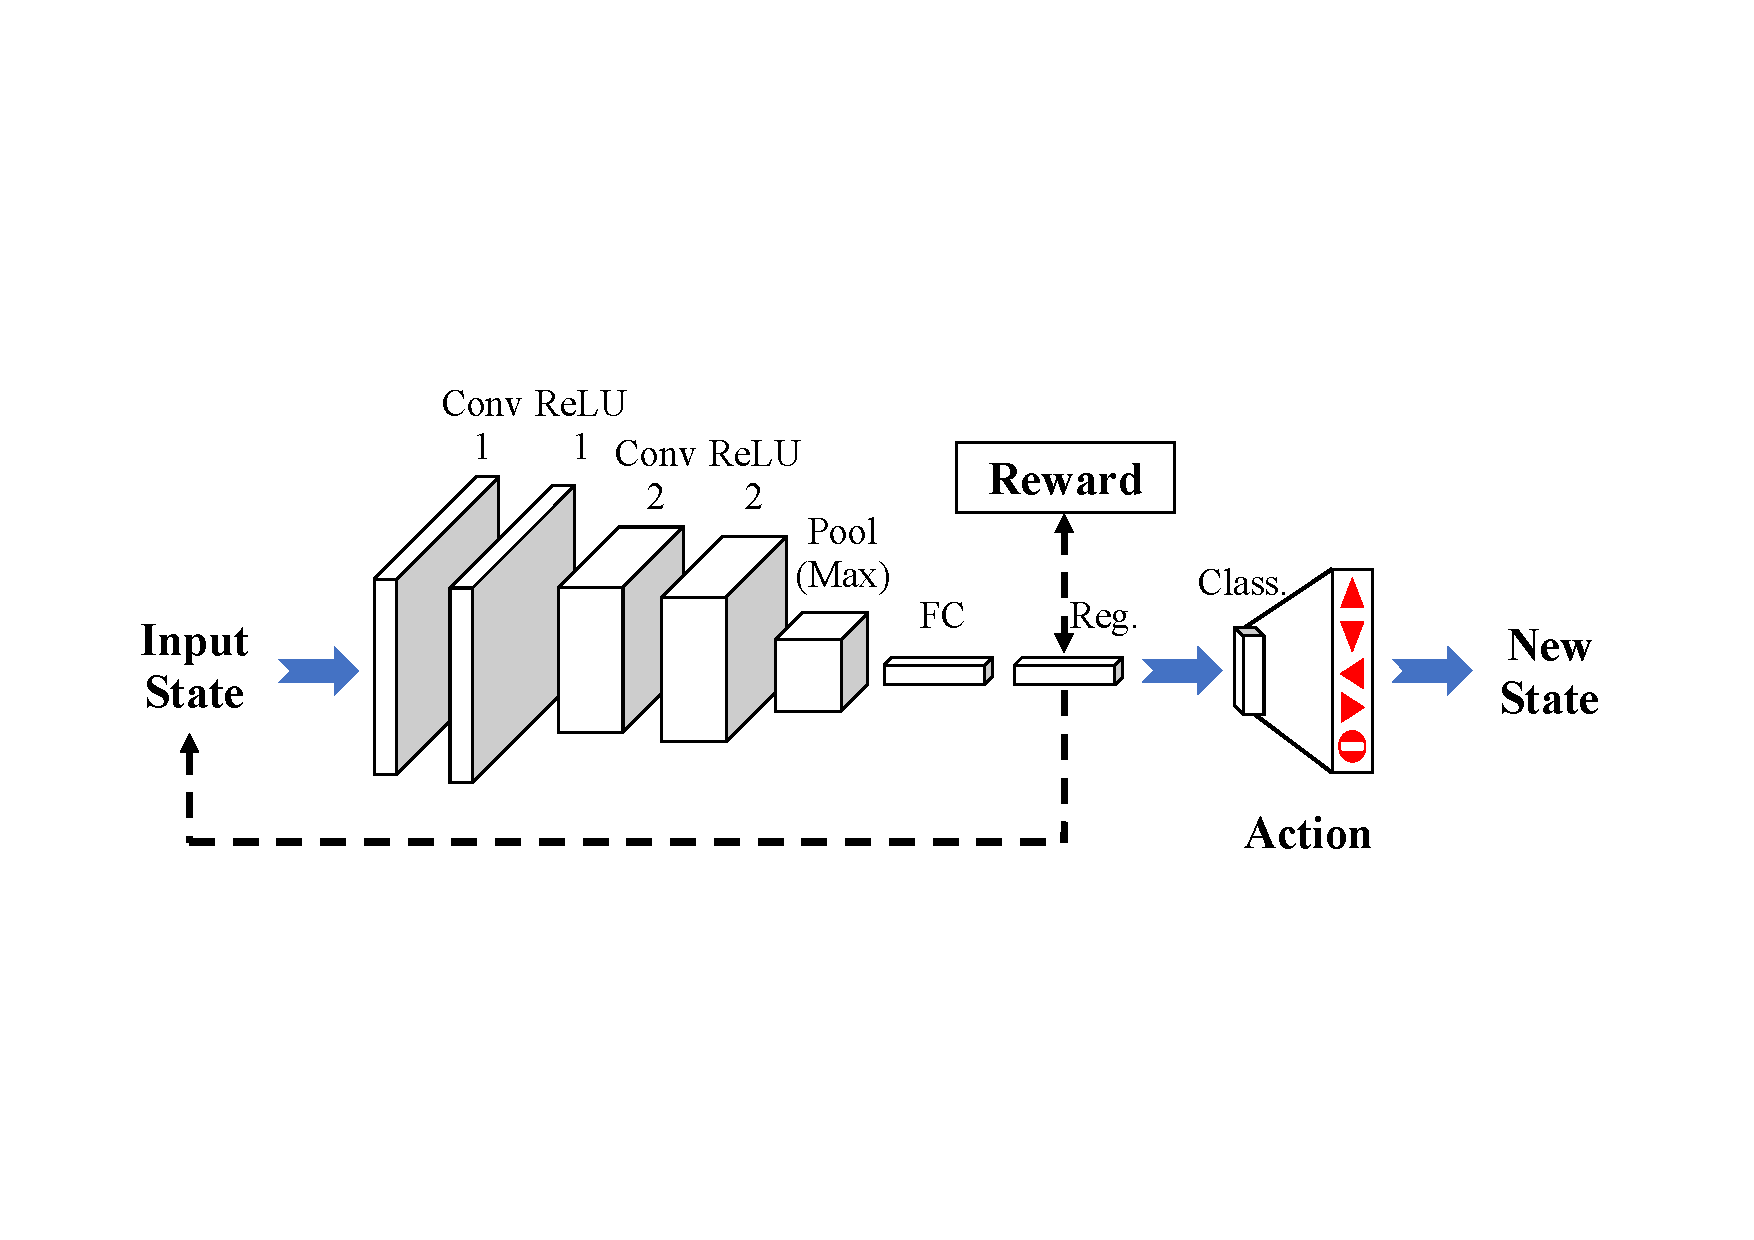
\includegraphics[scale=.65,trim=2cm 5.5cm 2cm 5.5cm,clip]{Deep_Reinf_Net1.pdf}
	\caption{The main design of the proposed DRL-RT. It consists of two conventional layers, two ReLU layers, a pooling layer, a fully connected layer, a regression layer and a classification layer}
	\label{Fig:Deep_Reinf_Net}
\end{figure*}
\section{\uppercase{Modelling}}
To model the road tracking, various essential issues have to be considered such as how to identify road crossing object(s), how to encode different tracking directions, how to design the deep reinforcement learning network to determine the next action, etc. Such issues will be illustrated and addressed in this section.

\subsection{Road Tracking:} 
Our research is based on the SYNTHIA-SEQS-05 database \cite{Ros2016TheSYNTHIA}. Video sequences were recorded and saved, from which one extracted front,  rear, left and right view road images around the car for both right and left steering cars. Each view covers a range of angle up to 100 degrees. As a result, a large number of simulated image frames were provided, each has a resolution of $760 \times 1,280 \times 3$ pixel. 

The images were taken in four different environments: clear
environment in spring, fog environment, rain environment and
heavy-rain environment.

In our study, we look at forward view road frames for a right steering car in all four environments. 

To differentiate the main objects on the road, specific colours were used, e.g., sky is grey, buildings are brown, roads are purple, side walks are blue and road markings are green. In other words, the purple and green colours refer to the allowed driving regions.  

More specifically, each view (image) can be divided into a safety zone and a danger zone. The safety zone is the zone that a car can keep moving to, as it is further away and it allows ample time to stop or slow down the car if necessary. The danger zone is the area that a car must stop if any objects are recognised. Such zones can be found in Fig. \ref{Fig:segmentation_regions1}. 

How do we determined a safe zone or a danger zone? In each image of Fig. \ref{Fig:segmentation}, a virtual triangle and trapezoid were drawn. The base of the triangle and trapezoid moves in the road direction, and the crossing lines can slope toward the tracking direction. The height of the triangle (and the trapezoid) is two thirds of the acquired image. The top one third of the trapezoid is the safety zone and the bottom two thirds is the danger zone. The shared point of the triangle and the trapezoid is called an anchor point. It denotes the road tracking direction. The anchor point can denote the direction by following the track centre. By drawing the virtual triangle in the trapezoid area is to specify three types of regions: left, right and centre. These regions can specify the direction of any crossing object. The car can, for instance, avoid an object crossing from the left side by moving to the right, if the space is empty there. If objects are identified from both sides in the danger zone, then the car has to stop.  

\subsection{Actions codes:} 
At any point, the following actions can be taken by a car: drive straight on, turn left or right, reverse and stop. In our work, we use a five-digit binary number to encode each action, see Table \ref{Table:Signs_codes}. The stop action is applied when the danger zone recognising object(s) in the way from both sides. 

When a crossing object is detected, it will change the action from that side with a ``0". For instance, the car is moving forward with action 01110, then an object appears in the danger zone from left, then the action becomes 00111. When another object appears from the right, the code will be 00110 and the car will stop. As long as there are no three consecutive 1's, the car has to stop.  We model all such cases as 00000 to reduce the number of coding values. Fig. \ref{Fig:segmentation} shows explanations for various coding cases.

The binary codes can be converted to desired equivalent codes. A standard conversion from the binary to decimal \cite{koren2001computer} is used. For instance, $(01110)_2=(14)_{10}$ and $(00111)_2=(7)_{10}$. The only exception here is the backward direction, where a negative sign (-) is added to refer to the reverse movement. It is worth mentioning that the reverse action can only be considered if the car is being out of the track. The road tracking actions with their suggested codes and descriptions are given in Table \ref{Table:Signs_codes}. The decimal codes are used in the regression layer of the proposed deep reinforcement learning network as will be explained later. They are referring to road tracking actions.

\begin{table}[!h]
	\centering
	\caption{The road tracking actions with their suggested codes and descriptions}
	\label{Table:Signs_codes}
	\begin{tabular}{|C{1.3cm}|C{1.3cm}|C{1.3cm}|C{2cm}|}
		\hline
		\textbf{Action sign} & \textbf{Binary code} & \textbf{Equivalent decimal code} & \textbf{Description} \\ \hline
		\begin{minipage}{.075\textwidth}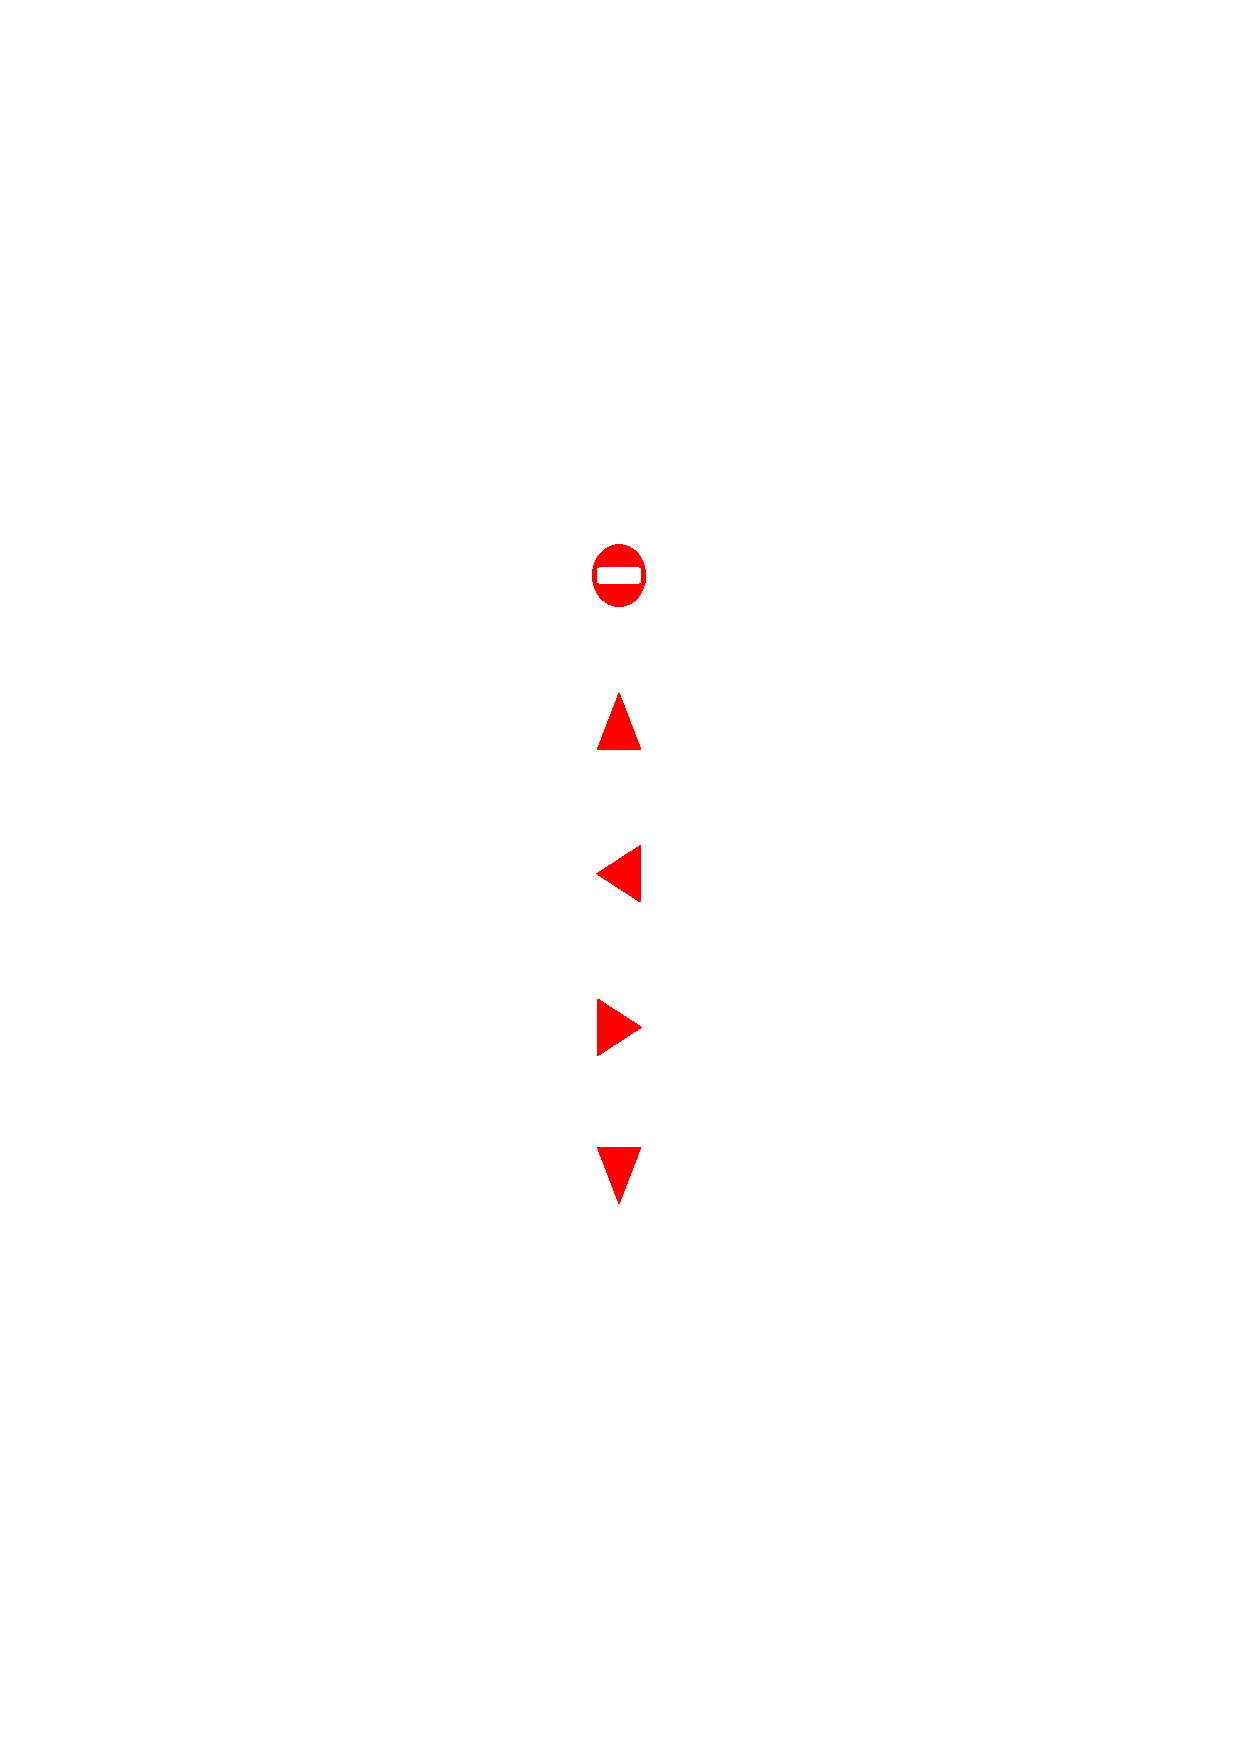
\includegraphics[scale=.5,trim=9.1cm 18.5cm 9.5cm 8cm,clip]{signs.pdf}\end{minipage}	& 0 0 0 0 0 & 0 & Stop (stop action because of crossing object(s)) \\ \hline
		\begin{minipage}{.075\textwidth}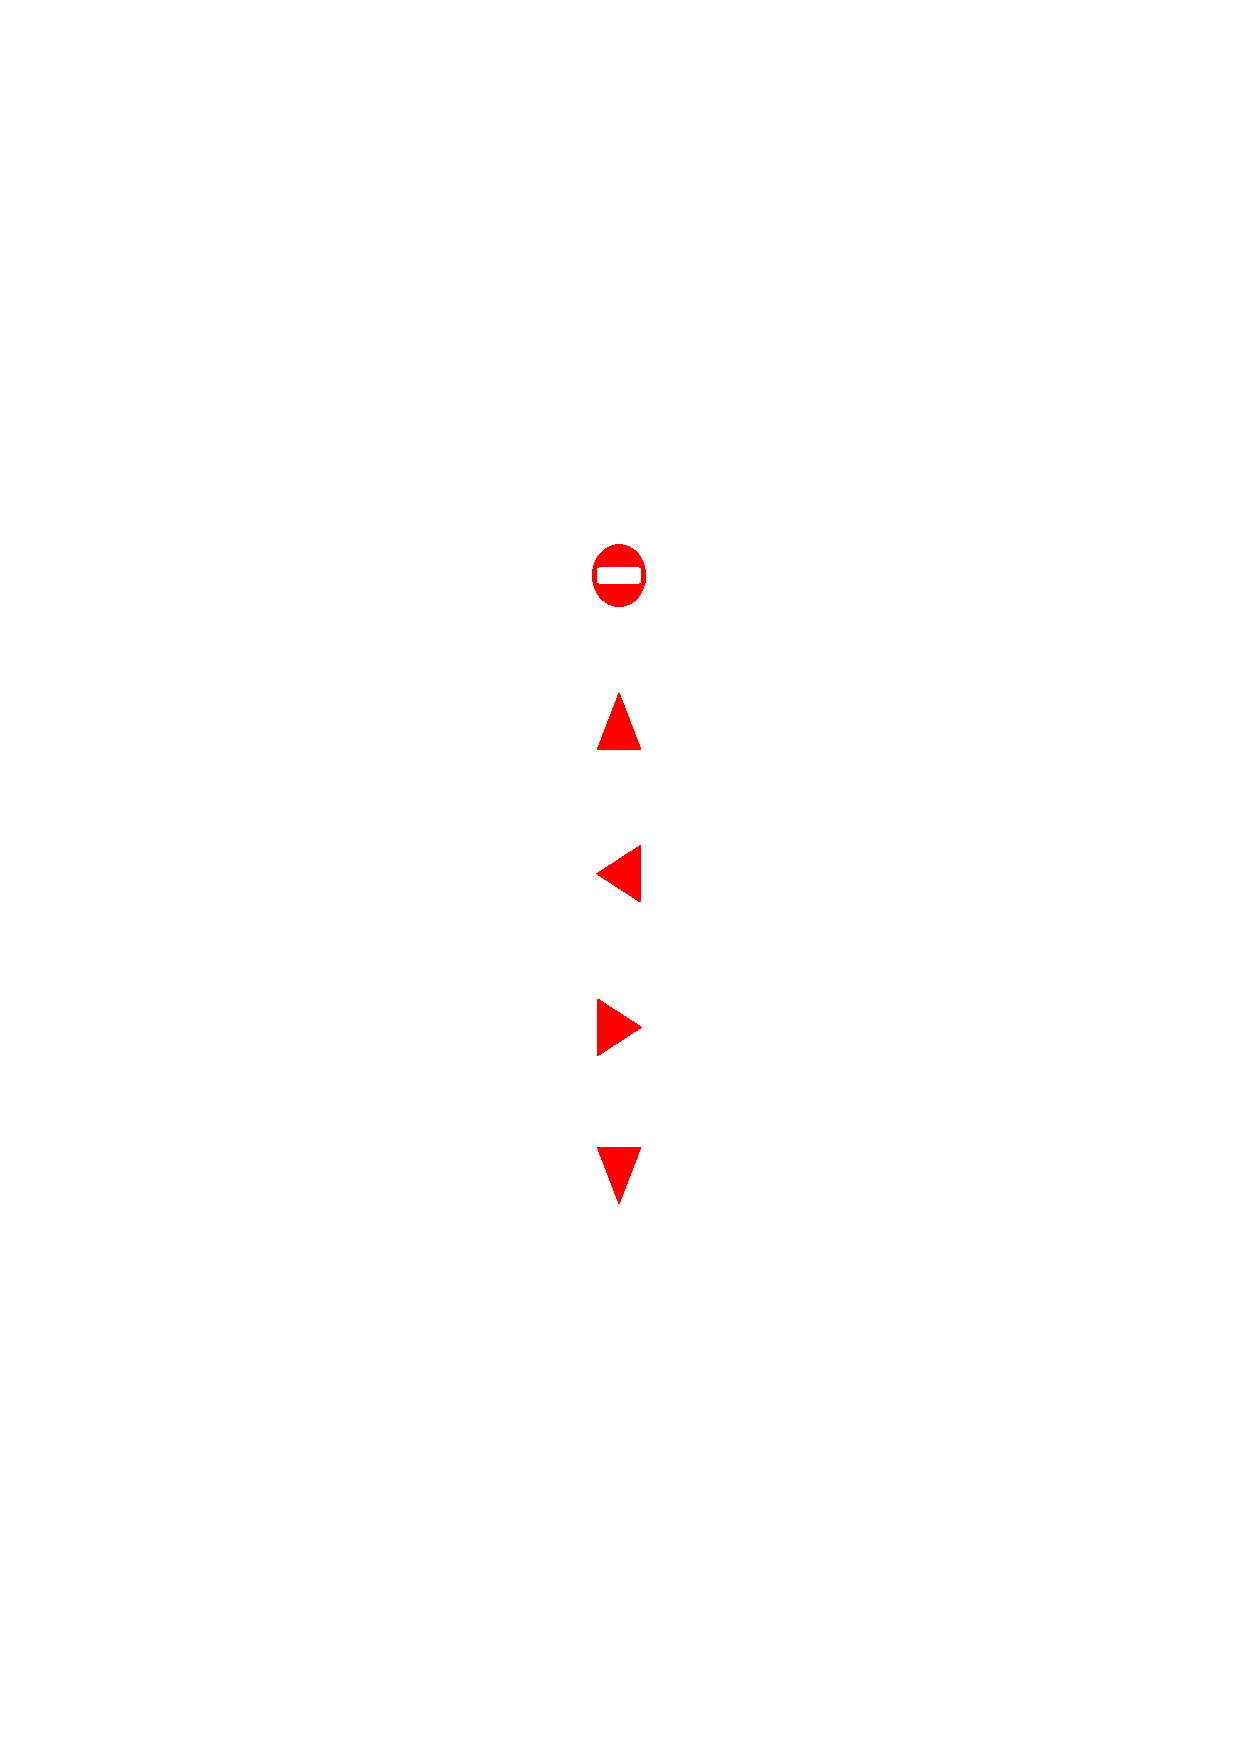
\includegraphics[scale=.5,trim=9.1cm 16cm 9.5cm 10.5cm,clip]{signs.pdf}\end{minipage}	& 0 1 1 1 0	& 14 & Move straight forward (follow the track to the forward direction) \\ \hline
		\begin{minipage}{.075\textwidth}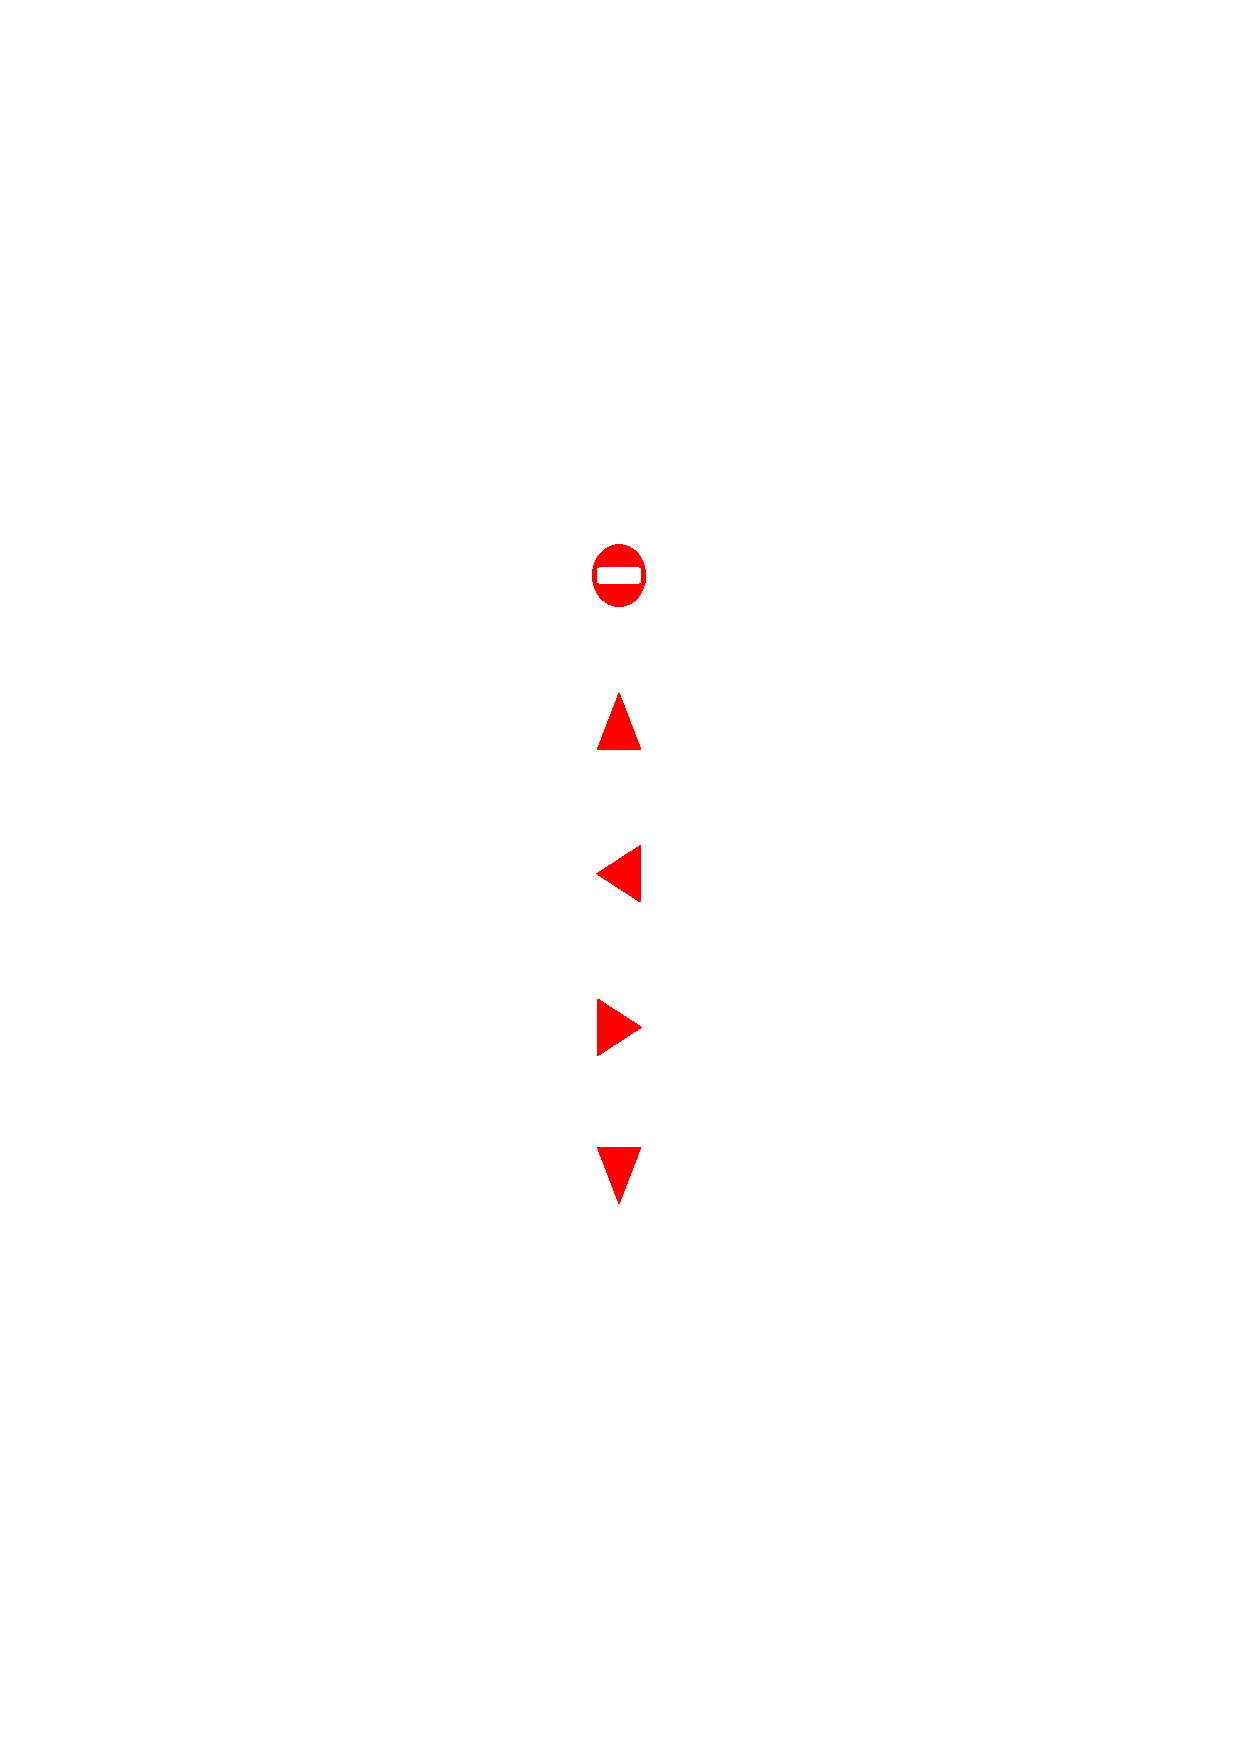
\includegraphics[scale=.5,trim=9.1cm 13.5cm 9.5cm 13cm,clip]{signs.pdf}\end{minipage}		& 1 1 1 0 0 & 28 & Move to the left (follow the track to the left direction) \\ \hline
		\begin{minipage}{.075\textwidth}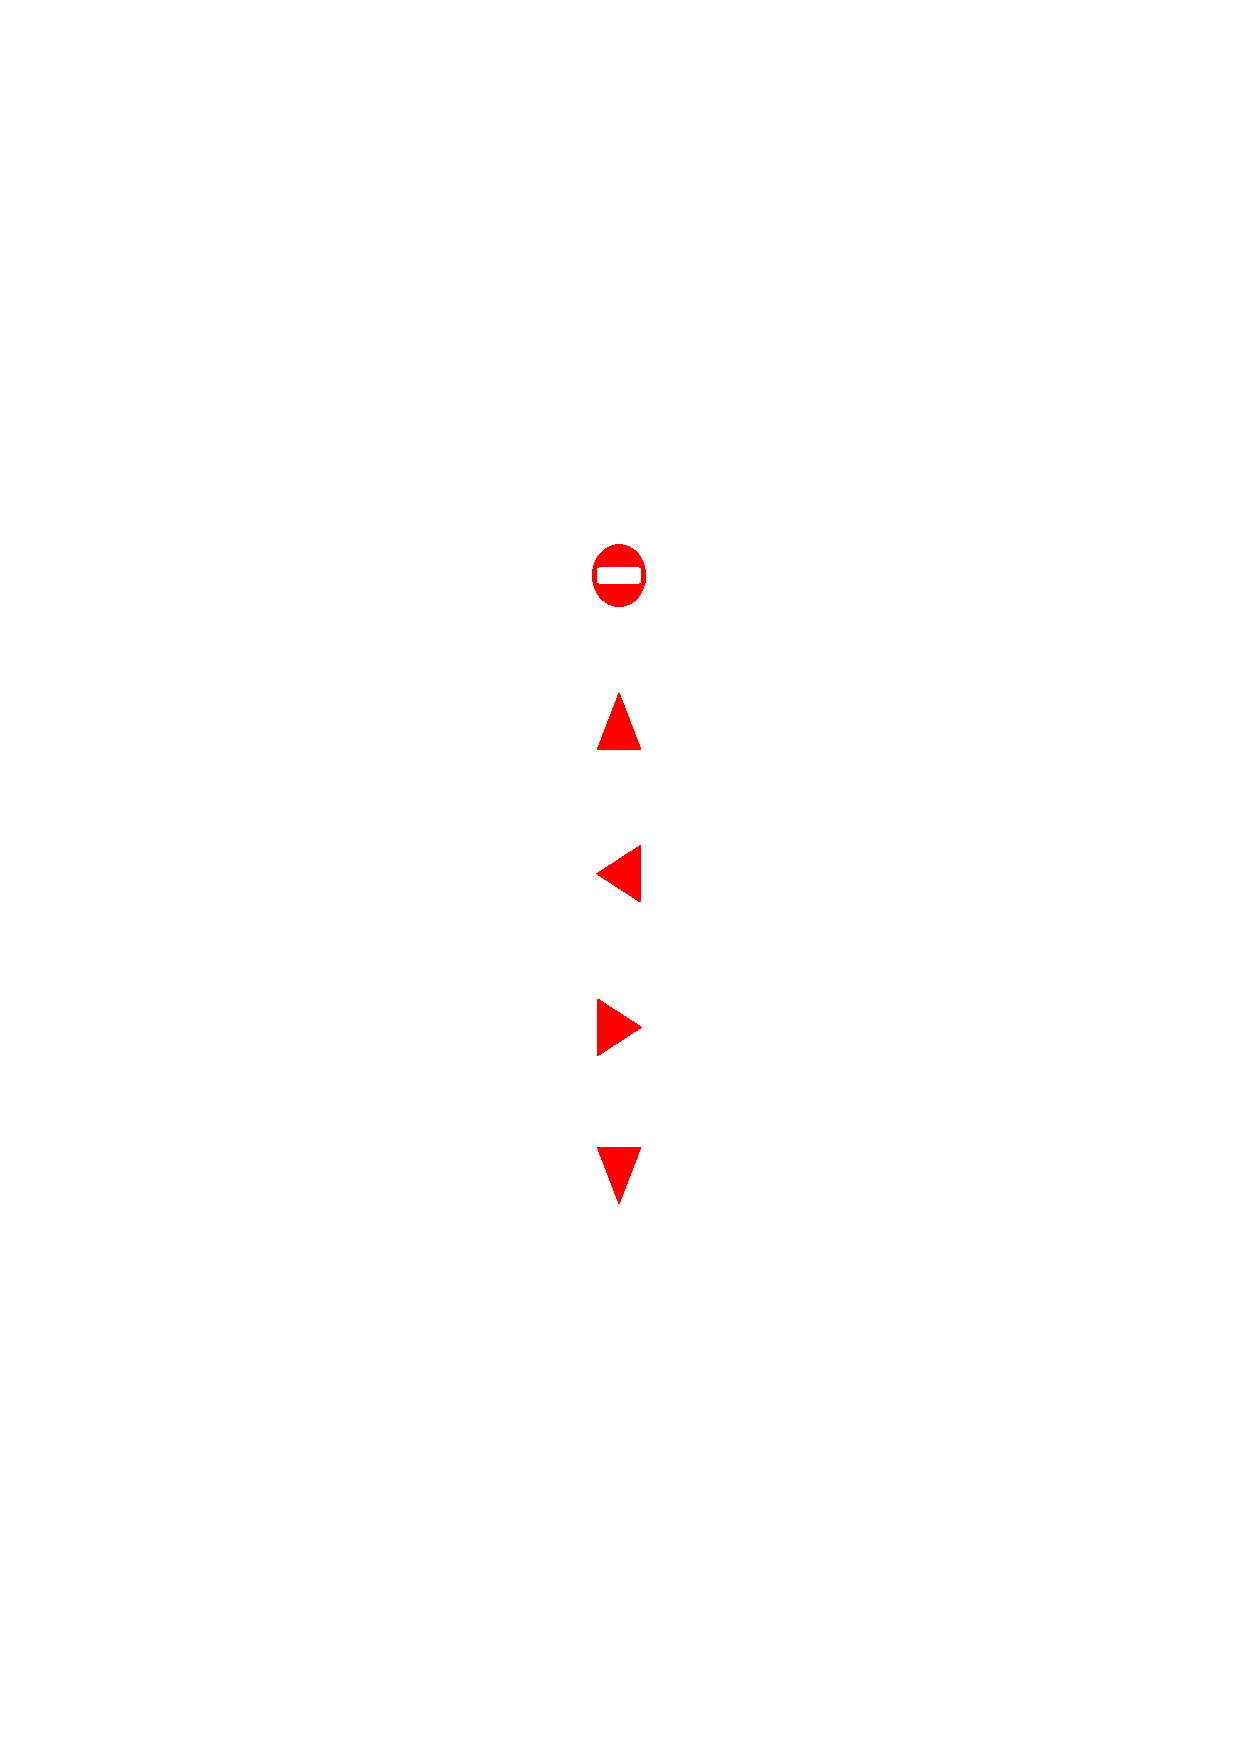
\includegraphics[scale=.5,trim=9.1cm 10.75cm 9.5cm 15.75cm,clip]{signs.pdf}\end{minipage}	& 0 0 1 1 1 & 7 & Move to the right (follow the track to the right direction) \\ \hline
		\begin{minipage}{.075\textwidth}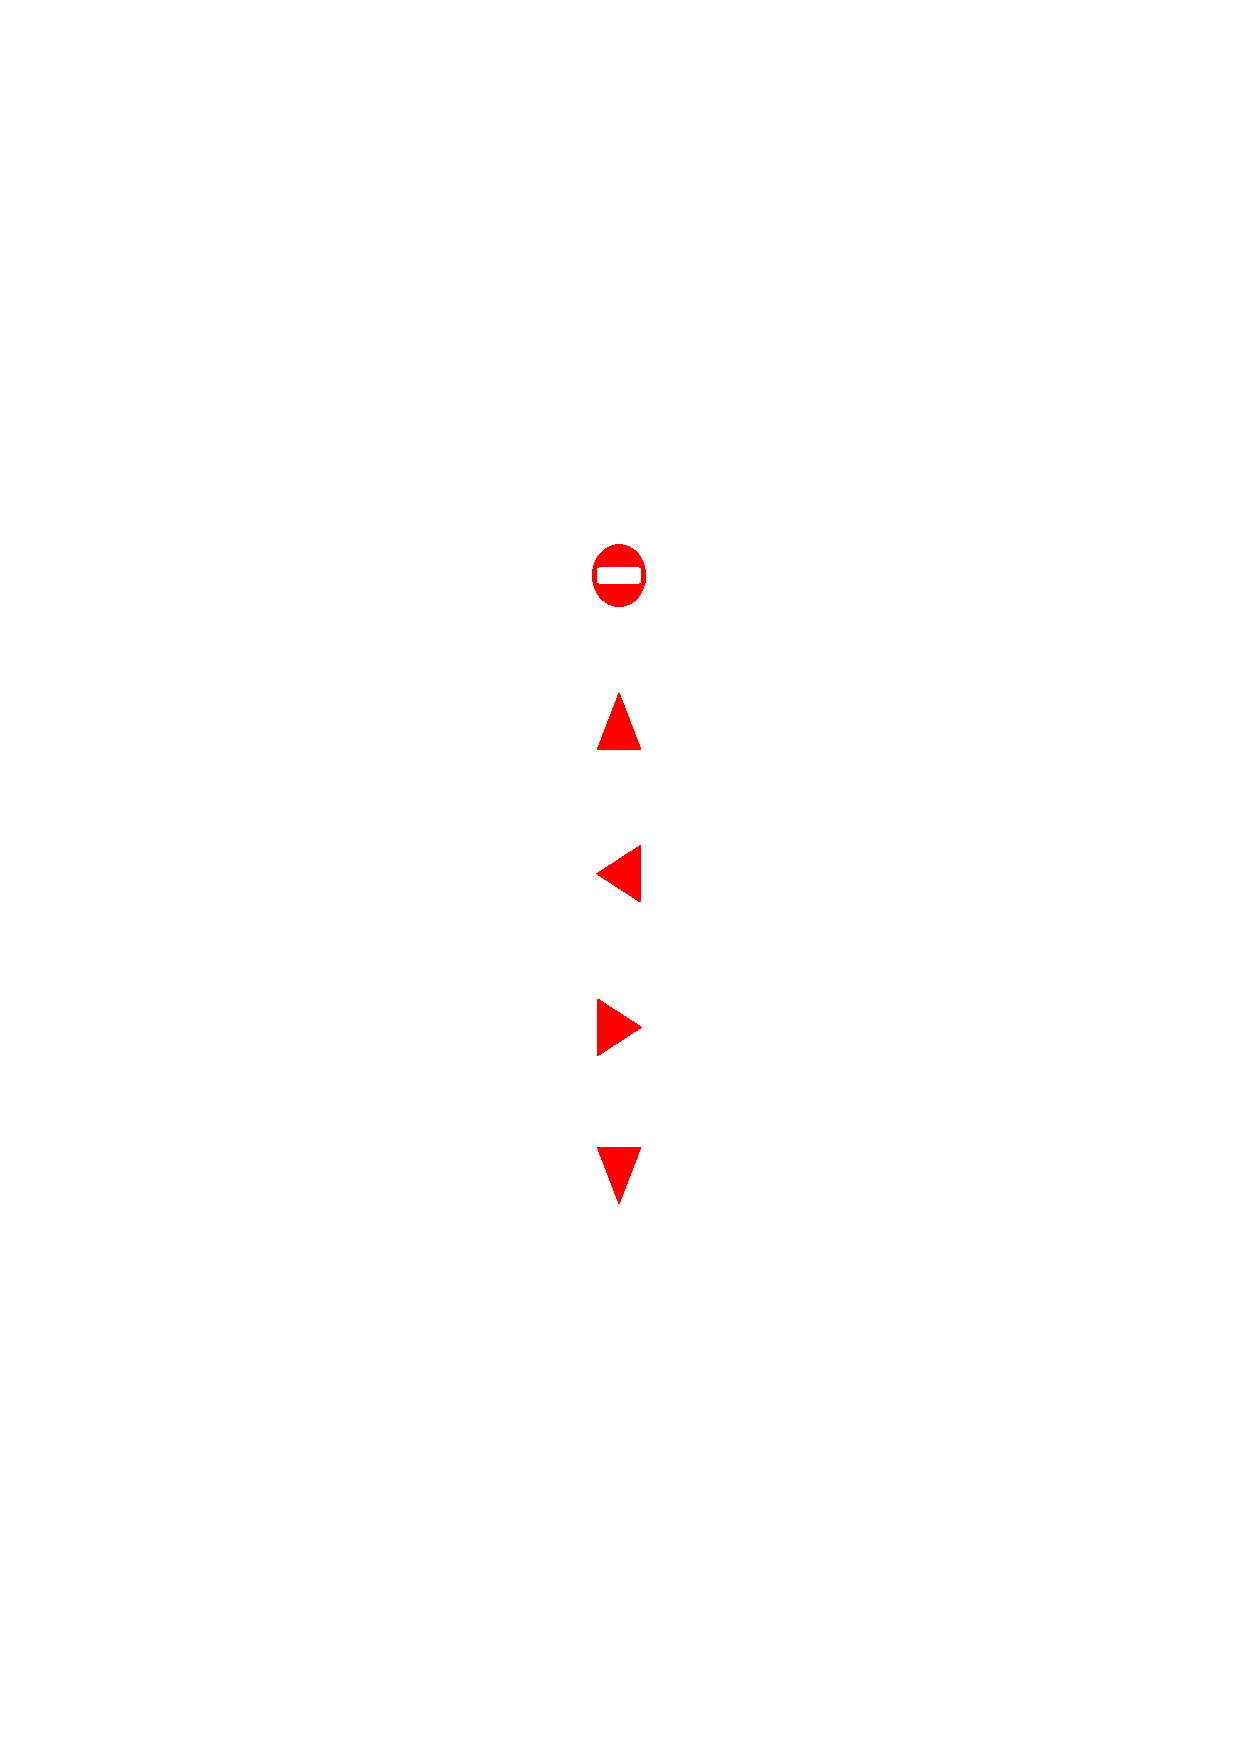
\includegraphics[scale=.5,trim=9.1cm 8.5cm 9.5cm 18cm,clip]{signs.pdf}\end{minipage} & 1 1 1 1 1 & -31 & Move backward (reverse moving to the back) \\ \hline
	\end{tabular}
\end{table}

\subsection{Policy search:} 
Principally, there are two essential types of reinforcement learning methods - policy search and value function. The first type refers to methods that consider searching for the optimal policy $\pi^*$. The second type refers to methods that consider investigating the optimal value-state function $V^*(s)$ \cite{Arulkumaran2017Deep}. In this work, the suggested DRL-RT network is based on the policy search. According to the MDP concept, the DRL-RT collects input images as current states $S_t$ and getting advantages from rewards $R$ to generate actions $A$, then the actions predict new states $S_{t+1}$. Consequently, the new states can be transitioned again in the inputs as current states. 

The essential equation of the policy search is demonstrated as:
\begin{equation}
\pi^*=\underset{\pi}{argmax}~\mathbb{E} [R\mid\pi]
\label{Eq:MDP}
\end{equation}
where $\pi$ is the policy and $\mathbb{E}$ is the expected return value \cite{arulkumaran2017brief}. In this work, the reward $R$ of the correct tracking is considered as (+1), whereas, the reward $R$ of the incorrect tracking is considered as (-1). Measuring the successful process of the road tracking will be based on obtaining as many positive rewards as possible. The discount factor $\gamma$ is considered here equal to (1).

\subsection{Proposed DRL-RT:} 
An applicable deep reinforcement network named the DRL-RT is established for road tracking. It consists of eight layers: two convention layers, two Rectified Linear Unit (ReLU) layers, a pooling layer, a fully connected layer, a regression layer and a classification layer. The input is an image of a car facing view, and it is considered as a current state. The input image size has been reduced to $254 \times 427 \times 3$ pixels in order to speed up the deep learning processes. The first layer after the input is a convolution layer, it consists of 5 filters each of which has a filter size of $10 \times 10$ pixels. This layer is important to extract the main features of the input images. A ReLU layer is used in the second layer. It removes the negative values and maintain the positive values of the previous layer. The third layer is also a convolution layer, it consists of 5 filters each of which has a filter size of $5 \times 5$ pixels. It extracts more features from the input images. A ReLU layer is employed again in the fourth layer. This layer rectifies the negative values. It has empirically been found that using two convolution layers with two ReLU layers can well analyse the information before being compressed by applying the next layer. Then, a pooling layer of a maximum type is applied in the fifth layer, the filter size here is $3 \times 3$ pixels with a stride of 3 pixels. The sixth layer is a fully connected layer, it collects the outputs from the previous layer and produces a series of decimal code tracking values. A regression layer is the seventh layer. In this layer, a series of directional road tracking codes are generated. The successful codes in this layer produce positive rewards, whereas, unsuccessful codes generate negative rewards. The network should be propagated, forwarded and backwarded the information for updating the network weights, during the training stage till obtaining as many positive rewards as possible. Given the codes in the regression layer, it is the classification layer's task to generate a new action - one of the five as in Table \ref{Table:Signs_codes}. Fig. \ref{Fig:Deep_Reinf_Net} shows the proposed DRL-RT network.

\subsection{Theoretical concepts:} 
The theoretical concepts of the main analysis layers (convolution, ReLU, pooling and fully connected) in the DRL-RT network were stated in \cite{omar2018deep}.

In the first and third layers, the collected information will be converted to feature maps. The feature map is defined as a convoluted 2D image with a kernel of weights. The following general equation represents the operations in a convolution layer:
\begin{equation}
z_{u,v,c^{l}}= \text{\footnotesize $B_{c^{l}}+\sum_{i=-k_h^{l}}^{k_h^{l}}\sum_{j=-k_w^{l}}^{k_w^{l}}\sum_{c^{l-1}=1}^{C^{l-1}} W_{i+k_h^{l},j+k_w^{l},c^{l-1}}^{c^{l}} z_{u+i,v+j,c^{l-1}}$}
\label{eq:conv_layer}
\end{equation}
where $z_{u,v,c^{l}}$ is a convolution layer outcome, $(u,v)$ is the assigned pixel, $c^{l}$ is the channel number of the convolution layer,  $W_{i,j,c^{l-1}}^{c^{l}}$ is the components of the kernel weights,  $B_{c^{l}}$ is the channel bias of the convolution layer, $k_h^l$ and $k_w^l$ are respectively the height and width of the kernel weights of the convolution layer, $C$ is the number of channels and it is here equal to 3 as we are using three channels of coloured images, $l-1$ is the previous layer, and $l$ is the current layer (the convolution layer) \cite{simo2016learning}. 
% \marginpar{Does it mean that all the $k_w^l$ are the same for all layers?}. Answer is: no and I have mentioned previously that $l$ represents the current layer.
%Again, this layer analyses the input values and produces FTs' feature maps.

A ReLU transfer function is applied in the second and fourth layers. This function can provide non-linear calculation to the DRL-RT. The ReLU function maintains the positive values and discards the negative values of a previous layer. Equation \eqref{eq:relu_layer} is exploited for the ReLU transfer function:
\begin{equation}
o_{u,v,c^{l}}=f(z_{u,v,c^{l}})=\max(0,z_{u,v,c^{l}})
\label{eq:relu_layer}
\end{equation}
where $o_{u,v,c^{l}}$ is a ReLU layer outcome and $\max$ is the maximum operation \cite{krizhevsky2012imagenet}. 

A pooling layer is used in the fifth part of the DRL-RT. The pooling layer can reduce the sizes of the feature maps. It obtains the maximum values from the last ReLU layer. In general, the pooling layer can be applied according to the following equation:
\begin{equation}
q_{a^{l},b^{l},c}=\underset{0\leq a<p_h,0\leq b<p_w}{\max} o_{a^{l}\times p_h+a,~b^{l}\times p_w+b,~c}
\label{eq:pooling_layer}
\end{equation}
where $q_{a^{l},b^{l},c}$ is a pooling layer outcome, $0\leq a^{l} <p_h^{l}$, $p_h^{l}$ is the height of the resulting feature maps, $0\leq b^{l} <p_w^{l}$, $p_w^{l}$ is the width of the resulting feature maps, $0\leq c <C^{l}=C^{l-1}$, $p_h$ and $p_w$ are respectively the width and height of the feature map sub-areas that require pooling \cite{wu2017introduction}. 

Subsequently, the fully connected layer is used to match between the designed number of subjects and the data of the pooling layer. Equation (\ref{eq:fully_connect}) demonstrates the fully connected layer processes:
\begin{equation}
g_{r}=\text{\footnotesize $\sum_{a=1}^{m_1^{l-1}} \sum_{b=1}^{m_2^{l-1}} \sum_{c=1}^{m_3^{l-1}} W_{a,b,c,r}^{l}(\textit{\textbf{Q}}_{c})_{a,b}~, ~~~~~~~\forall 1 \leq r \leq m^{l}$}
\label{eq:fully_connect}
\end{equation}
where $g_{r}$ is a fully connected layer outcome, $m_1^{l-1}$ and $m_2^{l-1}$ are the width and height of a feature map in the previous layer (the pooling layer) respectively, $m_3^{l-1}$ is the number of produced feature maps in the pooling layer, $W_{a,b,c,r}^{l}$ is the connection weights between the fully connected layer and the pooling layer, $\textit{\textbf{Q}}_{c}$ are the pooling layer outputs, and $m^{l}$ is the number of designed subjects \cite{stutz2014neural}.

The computations of the regression layer in the suggested DRL-RT network are based on the Mean Squared Error (MSE). The main MSE equation is illustrated as:
\begin{equation}
MSE=\frac{1}{n} \sum_{r=1}^{n}(t_r-g_r)^2
\label{eq:fully_connect}
\end{equation}
where $n$ is the number of computed values and $t$ is the desired output values \cite{saugirouglu2009intelligent}. If the regression output values close to the desired code values, positive rewards are produced. Otherwise, negative rewards are generated. 

Finally, the classification layer translates the regression information into actions by converting the obtained values into their assigned classes.

The MDP has been applied to the DRL-RT by providing current road tracking as current states $S_t$ to the input layer, estimating tracking directions as actions $A$, considering correct and incorrect tracking actions as rewards $R$, and predicting next tracking movements as new states $S_{t+1}$. Then, the new state (or next tracking view) are transitioned as a current state to the DRL-RT input layer in order to produce a new state again.
\begin{table*}[!t]
	\centering
	\caption{Examples of the four employed environments}
	\label{Table:Environments_Examples}
	\begin{tabular}{|C{1cm}|c|C{11.5cm}|}
		\hline
		\textbf{Database no.} & \textbf{Environment} & \textbf{Examples} \\ \hline
		(1)	& Spring & \begin{minipage}{.9\textwidth}\includegraphics[scale=.7,trim=2cm 24.5cm 2cm 2.5cm,clip]{examples.pdf}\end{minipage} \\ \hline
		%			&&\\ \hline
		(2) & Fog	& \begin{minipage}{.9\textwidth}\includegraphics[scale=.7,trim=2cm 20.5cm 2cm 6.5cm,clip]{examples.pdf}\end{minipage} \\ \hline
		%			&&\\ \hline
		(3)	& Rain &  \begin{minipage}{.9\textwidth}\includegraphics[scale=.7,trim=2cm 16.5cm 2cm 10.5cm,clip]{examples.pdf}\end{minipage} \\ \hline
		%			&&\\ \hline
		(4)	& Heavy- rain & \begin{minipage}{.9\textwidth}\includegraphics[scale=.7,trim=2cm 12.5cm 2cm 14.3cm,clip]{examples.pdf}\end{minipage} \\ \hline
		%			&&\\ \hline
	\end{tabular}
\end{table*}

\section{\uppercase{Results}}
\subsection{Databases:} 
Four databases from SYNTHIA \cite{Ros2016TheSYNTHIA} are used. The selected databases are constructed under different environment conditions: (1) spring, (2) fog, (3) rain and (4) heavy-rain. Moreover, their segmented images, which are provided by the same database, are found to be useful for manually determining the appropriate code of each track. Examples from the four databases are given in Table \ref{Table:Environments_Examples}.	

All implementations were performed by employing a computer with the following facilities: 8 GB RAM and Intel Core i5 processor (3.2 GHz). Only the microprocessor was used in this study to train and test the DRL-RT. The number of frames that have been utilized here are: 270, 284, 268 and 248 frames for the environments of spring, fog, rain and heavy-rain, respectively. The frames are equally divided between the training and testing stages (50\% each), where the odd frames are used in the training stage and the even frames are used in the testing stage.

\begin{figure}[!t]
	\centering
	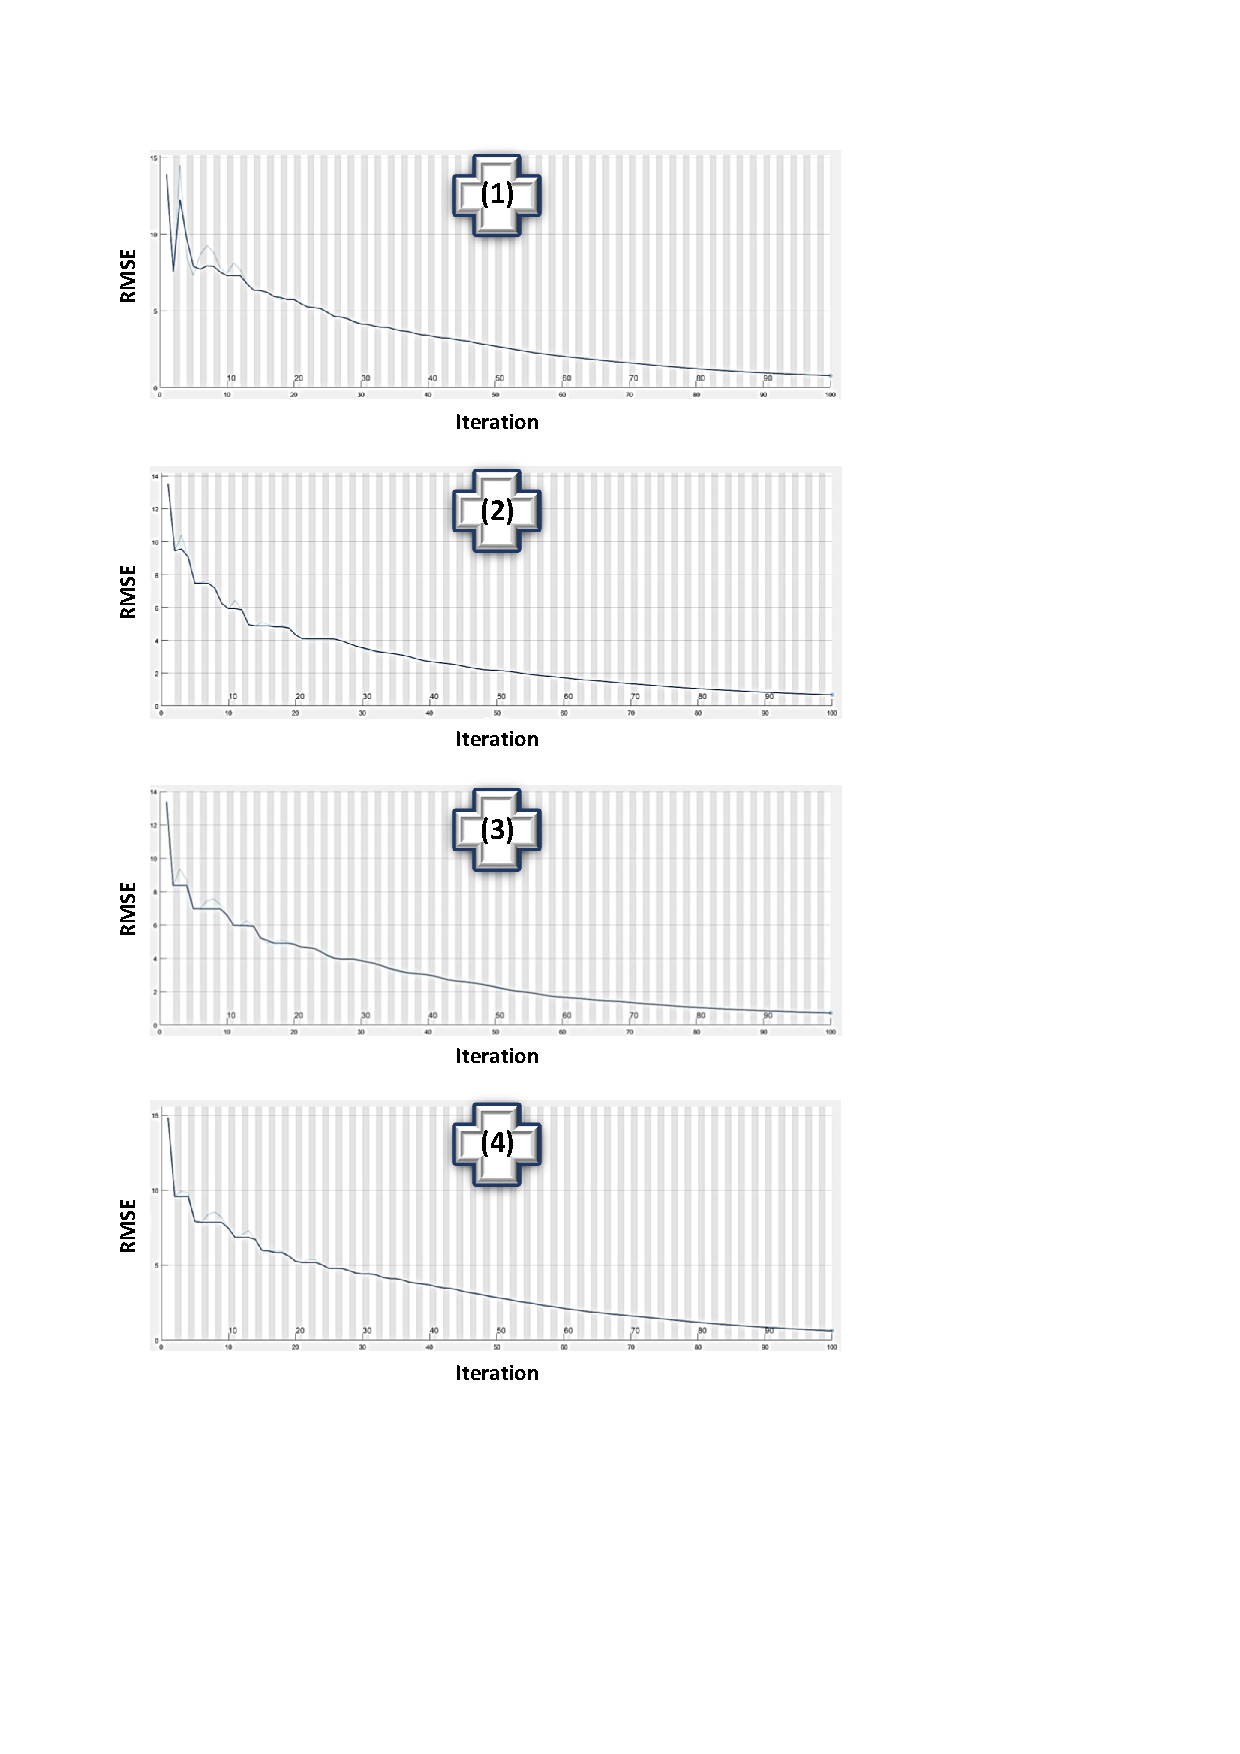
\includegraphics[scale=.6,trim=2cm 6cm 6.5cm 2cm,clip]{training_curves.pdf}
	\caption{The training performance of the DRL-RT for the: (1) spring environment, (2) fog environment, (3) rain environment and (4) heavy-rain environment}
	\label{fig:training_curves}
\end{figure}

\subsection{Training stage:} 
The suggested DRL-RT network has been separately trained for each environment. The following parameters have been assigned for the trainings: Adaptive Moment Estimation (ADAM) optimizer \cite{kingma2014adam}, learning rate equal to 0.0003, gradient decay factor ($\beta_1$) equal to 0.9, squared gradient decay factor ($\beta_2$) equal to 0.99 and mini batch size equal to 128. The training performance of the DRL-RT for the four databases are given in Fig. \ref{fig:training_curves}. This figure demonstrates the relationships between the Root Mean Square Error (RMSE) and the training iterations during the training stages. The RMSE values are usually exploited to demonstrate the differences between desired values and output values.	These differences are usually reduced during the proceeding of training itrations. Clearly, the curves are successfully declined toward goals.

\subsection{Testing stage:} 
The results of the testing stages are interested as it can be observed in Fig. \ref{fig:Main_Results}. To illustrate, the driving accuracy attained its highest value of 93.94\% by using the spring environment database. This is because that the DRL-RT has analysed very clear provided images.  The fog environment database obtained a high driving accuracy of 93.66\%. Here, the overall views are blurred but the road tracking can still be distinguished. The DRL-RT could recognize the road tracking but with slightly lower accuracy than the spring views. The driving accuracy of the rain environment database achieved 89.55\% and this is due to the noise effects of rain drops on image views. Finally, the inferior driving accuracy of 84.68\% was recorded for the heavy-rain environment database as the amount of rain drops (or noise) are increased here.
\begin{figure}[!t]
	\centering
	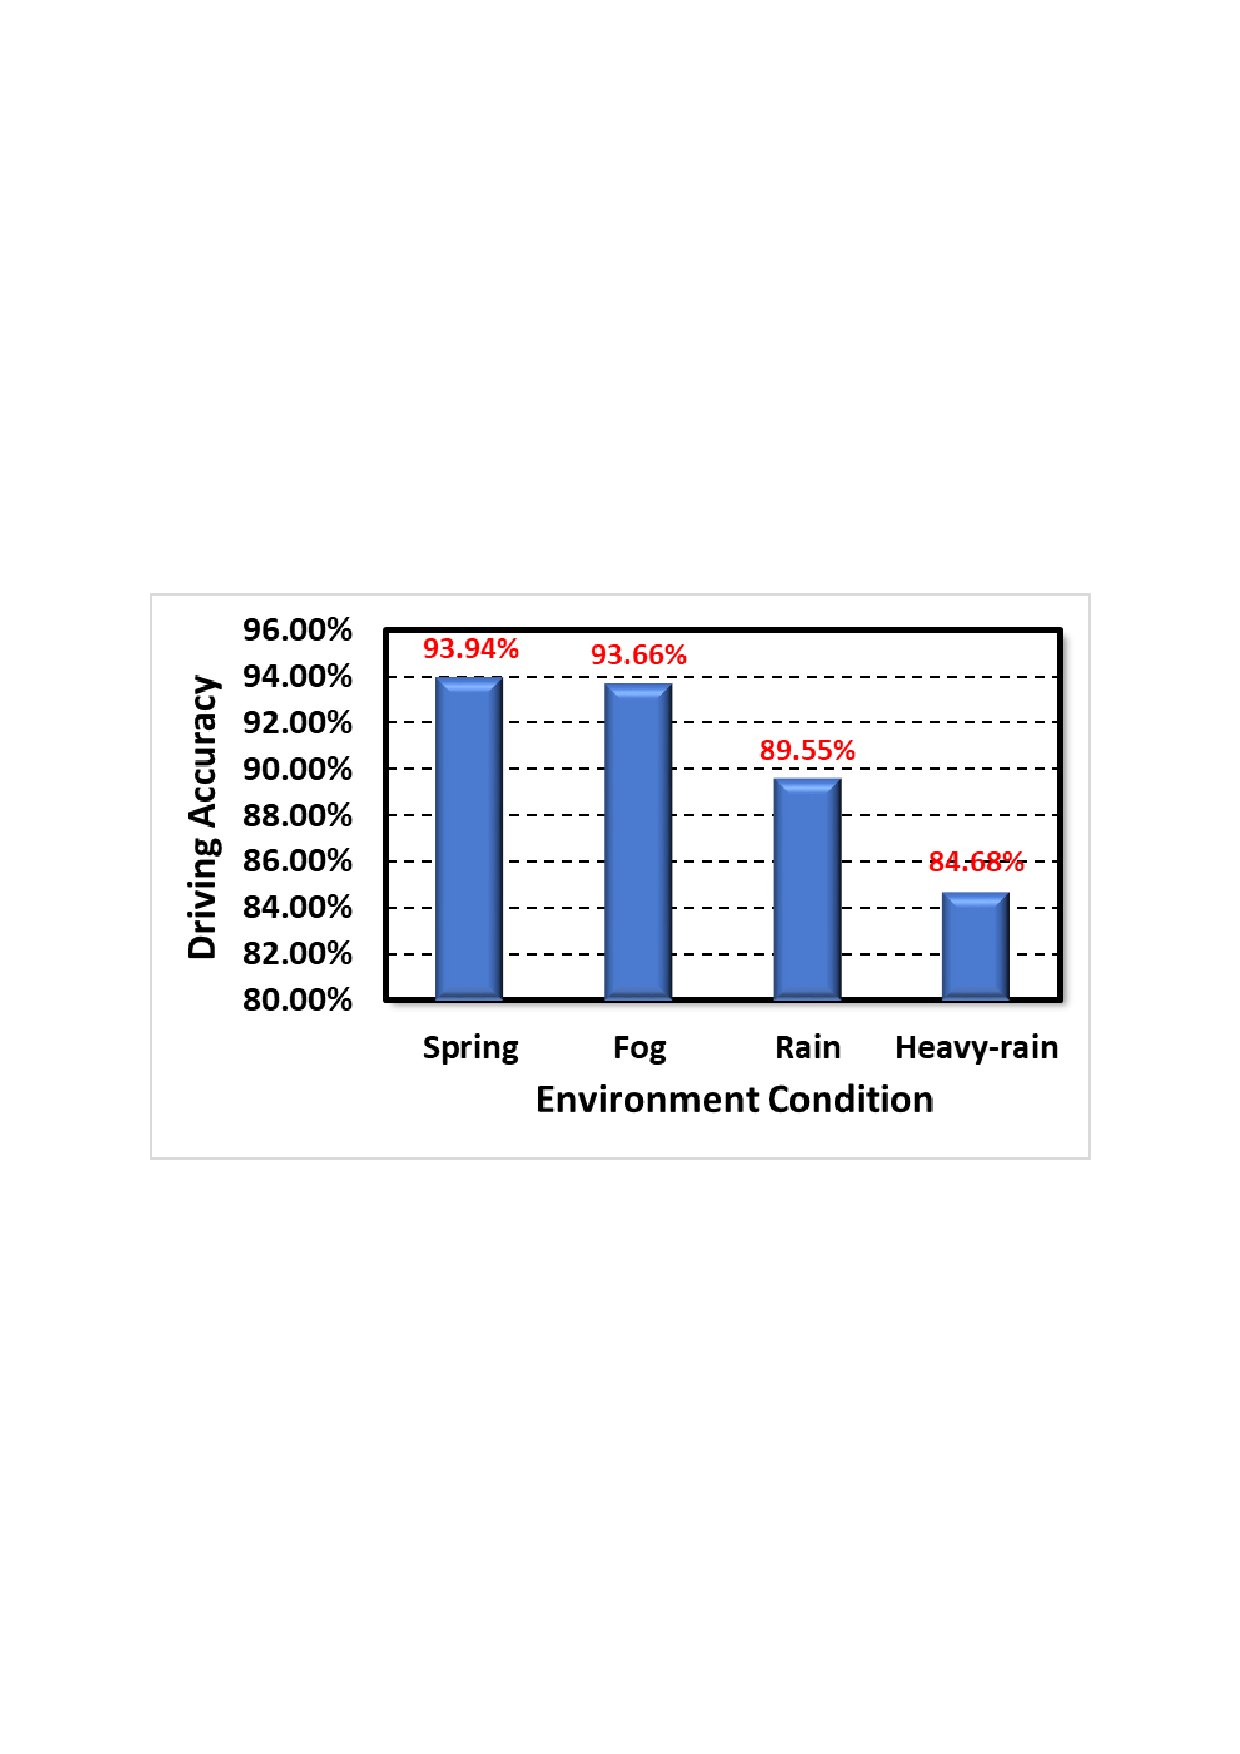
\includegraphics[scale=.5,trim=3cm 10.3cm 2.7cm 10.3cm,clip]{Main_Results.pdf}
	\caption{The performance of the DRL-RT under different employed environments}
	\label{fig:Main_Results}
\end{figure}

\subsection{Comparisons:} 
In the case of comparisons, hard efforts were performed to investigate and simulate various deep learning approaches. Comparisons have been established between our proposed DRL-RT method and other suggested networks. Table \ref{Table:Comparisons} shows the accuracies of different deep learning networks by applying the database of SYNTHIA-SEQS-05-SPRING, some parameters were reasonably changed to allow acceptable comparisons. The reason of selecting this database here is that it has the clear environment, which is suitable to discard undesired effects and provide fair judgement.

\begin{table}[]
	\centering
	\caption{A comparison between our proposed DRL-RT method and other suggested networks}
	\label{Table:Comparisons}
	\begin{tabular}{|C{3cm}|C{2cm}|c|}
		\hline
		\textbf{Reference} & \textbf{Deep learning method} & \textbf{Accuracy} \\ \hline
		Karaduman and Eren \cite{Karaduman2017Deep} & CNN & 67.42\% \\ \hline
		Bojarski \textit{et al.} \cite{bojarski2016end} & CNN & 74.24\% \\ \hline
		George and Routray \cite{George2016Real} & CNN & 83.33\% \\ \hline
		Yun \textit{et al.} \cite{Yun2017Action,Yun2018Action} & ADNet & 83.33\% \\ \hline
		Mnih \textit{et al.} \cite{mnih2015human} & DQN & 88.64\% \\ \hline
		Proposed method & DRL-RT & 93.94\% \\ \hline
	\end{tabular}
\end{table}

From Table \ref{Table:Comparisons}, it can be seen that the suggested CNN in \cite{Karaduman2017Deep} obtained the inferior tracking accuracy of 67.42\%. This is due to the architecture of this network, where it constructed to classify directions of traffic signs. More specifically, a pooling layer was applied after each convolution layer and no ReLU layers were used. This caused compressing and wasting useful extracted features after each convolution layer. The CNN which is used in \cite{bojarski2016end} attained a low accuracy of 74.24\%. The main drawback of this network is that it considers steering angles to be tracked, where this increases the erroneous of obtaining precise outputs. The CNN in \cite{George2016Real} achieved 83.33\%. This is also due to the architecture of this network, which was designed for classifying eye gaze directions. The ADNet which was approached in \cite{Yun2017Action,Yun2018Action} attained the same accuracy of 83.33\%. 
%	The architecture of this network was mainly consists of convolution layers and fully connected layers, this seems not 
The essential problem here is represented by the considered rewards, which were basically designed %after moving objects and not during the moving. 
for recognizing moved objects as the rewards are updated in the stop action. In addition, the Adnet architecture is not so appropriate for road tracking tasks. The Deep Q-Network (DQN), which is proposed in \cite{mnih2015human} and illustrated in \cite{arulkumaran2017brief} achieved reasonable accuracy of 88.64\%. This can be due to the DQN processes, where it combines between the deep network and the Q-learning. This network can be considered as the nearest method to our approach. Finally, our proposed method has shown superior performance by attaining the accuracy of 93.94\%. This can be due to the overall structure of our road tracking method including the network architecture, tracking policy and designed codes.

\section{\uppercase{Conclusion}}
A deep reinforcement neural network is established for road tracking termed the DRL-RT. This network is suggested to guide driving cars under different weather environments. Different tracking instances were coded to represent the appropriate road tracking. The MDP concept is used here, where the network accepted states and produced actions by taking advantages from rewards. The proposed deep reinforcement network is based on the policy search. This study were compared with other work and it reported superior performance. In addition, interesting results were benchmarked by the proposed approach. That is, the best performance of 93.94\% was recorded for a clear environment and reasonable performance were reported under unclear environments of fog, rain and heavy-rain as the obtained accuracies were respectively equal to 93.66\%, 89.55\% and 84.68\%. 

\section*{\uppercase{Acknowledgment}}
$\bullet$ ``RC grant EP/P015387/1".
	
	
	\bibliographystyle{apalike}
	{\small
		\bibliography{references14}}
	
\end{document}

